\section{Aufbau und Durchführung}
Der verwendete Versuchsaufbau ist in Abbildung \ref{fig:aufbau} dargestellt. Die Kupferprobe befindet sich in einem Rezipienten,
welcher sich in einem Dewargefäß befindet. Zur Kühlung des Rezipienten wird das Dewargefäß mit flüssigem Stickstoff befüllt. Um Energieverluste
durch Wärmetransport während der Messung zu verhindern, wird der Rezipient mithilfe einer Vakuumpumpe evakuiert. Da Wärmestrahlung nicht verhindert werden kann,
befindet sich die Probe in einem Kupferzylinder, der immer auf der gleichen Temperatur gehalten wird wie die Probe, sodass dieser die gleiche Energie an die Probe
zurückstrahlt, die diese abgibt. Die Kupferprobe und der Kupferzylinder besitzen beide jeweils eine Heizwicklung und einen Pt-100-Widerstand zur Messung der Temperatur.
Da die Widerstände temperaturabhängig sind, lässt sich durch Messung des Widerstands die Temperatur der Probe berechnen.

\begin{figure}[h]
  \centering
  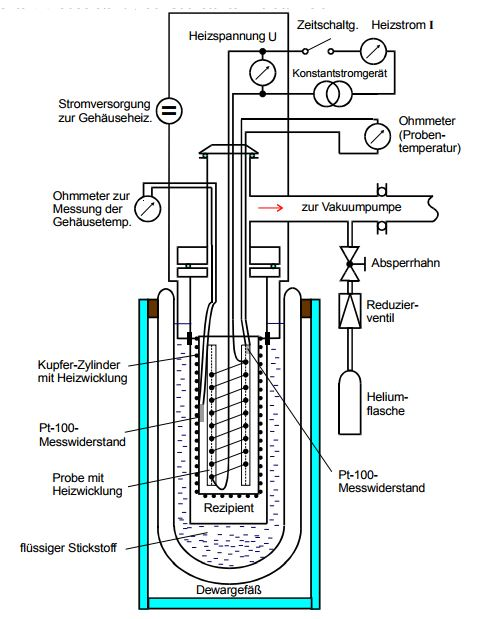
\includegraphics[scale=0.7]{graphics/Aufbau.jpg}
  \caption{Schematischer Versuchsaufbau \cite{anleitung}.}
  \label{fig:aufbau}
\end{figure}

Vor der Messung wird der Rezipient mit flüssigem Stickstoff auf ca. $\SI{80}{K}$ runtergekühlt. Dazu wird der Rezipient zunächst evakuiert und dann mit Helium gefüllt,
um den Wärmeaustausch innerhalb des Rezipienten zu fördern. Nach der Kühlung wird der Rezipient wieder evakuiert und die Messung begonnen. Zur Messung der Molwärme wird
die Kupferprobe elektrisch geheizt. Aus der Dauer des Heizvorgangs, der Spannung und der Stromstärke lässt sich die zugeführte Energie ermitteln und aus der erzeugten
Temperaturdifferenz lässt sich dann die Molwärme berechnen. Die Messung wird in Intervallen mit einer Temperaturdifferenz zwischen $\SI{7}{K}$ und $\SI{11}{K}$ durchgeführt,
bis die Probe eine Temperatur von etwa $\SI{300}{K}$ erreicht hat.
